%%%%%%%%%%%%%%%%%%%%%%%%%%%%%%%%%%%%%%%%%%%%%%%%%%%%%%%%%%%%%%%%%%%%%%%%%%%%%%%%
%%%%%%%%%%%%%%%%%%%%%%%%%%%%%%%%%%%%%%%%%%%%%%%%%%%%%%%%%%%%%%%%%%%%%%%%%%%%%%%%
%
% A general frame for lecture slides and lecture notes in one file
% using LaTeX beamer
%
%%%%%%%%%%%%%%%%%%%%%%%%%%%%%%%%%%%%%%%%%%%%%%%%%%%%%%%%%%%%%%%%%%%%%%%%%%%%%%%%
%%%%%%%%%%%%%%%%%%%%%%%%%%%%%%%%%%%%%%%%%%%%%%%%%%%%%%%%%%%%%%%%%%%%%%%%%%%%%%%%
\documentclass[ignorenonframetext,11pt]{beamer}
%\usepackage[ngerman]{babel}
%\usepackage[T1]{fontenc}
\usepackage[utf8]{inputenc}
\usepackage{lmodern}
\usepackage{amsmath,amssymb,amsfonts}


% only presentation 
\mode<presentation>
{
  \usetheme{default}
%  \usecolortheme{crane}
  \setbeamercovered{transparent}
%  \setlength{\parindent}{0pt}
%  \setlength{\parskip}{1.35ex plus 0.5ex minus 0.3ex}
%  \usefonttheme{structuresmallcapsserif}
  \usefonttheme{structurebold}
  \setbeamertemplate{theorems}[numbered]
  \usepackage{amscd}
}

% all after
\usepackage{tikz} 
\usetikzlibrary{patterns}
\usepackage{pgfplots,adjustbox}
\usepackage{eurosym} 
\usepackage{graphicx}
\usepackage{multimedia}
\usepackage{psfrag}
\usepackage{listings}
\lstset{language=C++, basicstyle=\ttfamily, 
  keywordstyle=\color{black}\bfseries, tabsize=4, stringstyle=\ttfamily,
  commentstyle=\it, extendedchars=true, escapeinside={/*@}{@*/}}
\usepackage{curves}
%\usepackage{epic}
\usepackage{calc}
%\usepackage{picinpar}
%\usepackage{fancybox}
%\usepackage{xspace}
\usepackage{enumerate}
\usepackage{algpseudocode}
\usepackage{color}
\usepackage{bold-extra}
\usepackage{bm}
\usepackage{stmaryrd}
%\usepackage[squaren]{SIunits}
\usepackage{nicefrac}

\usepackage{fancyvrb,bbm,xspace}
\usepackage{lmodern}
\usepackage{fancyvrb,bbm,xspace}
\usepackage[binary-units]{siunitx}
\usepackage{xcolor,tabu}

\definecolor{niceblue}{rgb}{0.122,0.396,0.651}   %% 31, 101, 166 or #1F65A6
\definecolor{niceorange}{RGB}{255,205,86}        %% #FFCD56
\definecolor{nicered}{RGB}{220,20,60}                      %% rgb(220, 20, 60)
\definecolor{niceteal}{HTML}{00A9AB}
\definecolor{niceviolet}{HTML}{820080}

\definecolor{niceblueLight}{HTML}{91CAFB}
\definecolor{niceblueVeryLight}{HTML}{DDEFFF}

\usepackage{dsfont}

%\newcommand{\hlineabove}{\rule{0pt}{2.6ex}}
%\newcommand{\hlinebelow}{\rule[-1.2ex]{0pt}{0pt}}

%\usecolortheme[RGB={37,75,123}]{structure}
% \definecolor{structurecolor}{rgb}{0.905,0.318,0.071}

% \setbeamercolor{frametitle}{fg=black,bg=}
% \setbeamercolor{sidebar left}{fg=,bg=}

% \setbeamertemplate{headline}{\vskip4em}
% \setbeamersize{sidebar width left=.9cm}

% \setbeamertemplate{navigation symbols}{}
%\setbeamertemplate{blocks}[rounded][shadow=true]
%\setbeamertemplate{itemize items}[square]

\mode<presentation> 
{
\theoremstyle{definition}
}
\newtheorem{Def}{Definition}%[section]
\newtheorem{Exm}[Def]{Example}
\newtheorem{Lem}[Def]{Lemma}
\newtheorem{Rem}[Def]{Remark}
\newtheorem{Rul}[Def]{Rule}
\newtheorem{Thm}[Def]{Theorem}
\newtheorem{Cor}[Def]{Corollary}
\newtheorem{Obs}[Def]{Observation}
\newtheorem{Ass}[Def]{Assumption}
\newtheorem{Pro}[Def]{Property}
\newtheorem{Alg}[Def]{Algorithm}
\newtheorem{Prp}[Def]{Proposition}
\newtheorem{Lst}[Def]{Listing}

% Delete this, if you do not want the table of contents to pop up at
% the beginning of each subsection:
\AtBeginSection[]
{
  \begin{frame}<beamer>
    \frametitle{Contents}
    \tableofcontents[sectionstyle=show/shaded,subsectionstyle=hide/hide/hide]
%\tableofcontents[currentsection]
  \end{frame}
}

% Title definition
\mode<presentation>
{
  \title{DUNE PDELab Tutorial 02\\
  {\small  The Cell-centered Finite Volume Method}}
  \author{Peter Bastian}
  \institute[]
  {
   Interdisziplinäres Zentrum für Wissenschaftliches Rechnen\\
   Im Neuenheimer Feld 368, D-69120 Heidelberg \\[6pt]
  }
  \date[\today]{\today}
}


% logo nach oben
\mode<presentation>
{
% No navigation symbols and no lower logo
\setbeamertemplate{sidebar right}{}

% logo
\newsavebox{\logobox}
\sbox{\logobox}{%
    \hskip\paperwidth%
    \rlap{%
      % putting the logo should not change the vertical possition
      \vbox to 0pt{%
        \vskip-\paperheight%
        \vskip0.35cm%
        \llap{\insertlogo\hskip0.1cm}%
        % avoid overfull \vbox messages
        \vss%
      }%
    }%
}

\addtobeamertemplate{footline}{}{%
    \usebox{\logobox}%
}
}

%%%%%%%%%%%%%%%%%%%%%%%%%%%%%%%%%%%%%%%%%%%%%%%%%%%%%%%%%%%%%%%%%%%%%%%%%%%%%%%%
%%%%%%%%%%%%%%%%%%%%%%%%%%%%%%%%%%%%%%%%%%%%%%%%%%%%%%%%%%%%%%%%%%%%%%%%%%%%%%%%
%
% now comes the individual stuff lecture by lecture
%
%%%%%%%%%%%%%%%%%%%%%%%%%%%%%%%%%%%%%%%%%%%%%%%%%%%%%%%%%%%%%%%%%%%%%%%%%%%%%%%%
%%%%%%%%%%%%%%%%%%%%%%%%%%%%%%%%%%%%%%%%%%%%%%%%%%%%%%%%%%%%%%%%%%%%%%%%%%%%%%%%

\begin{document}

\frame{\titlepage}

%%%%%%%%%%%%%%%%%%%%%%%%%%%%%%%%%%%%%%%%%%%%%%%%%%%%%%%%%%%%%%%%%%%%%%%%%%%%%%%%
%%%%%%%%%%%%%%%%%%%%%%%%%%%%%%%%%%%%%%%%%%%%%%%%%%%%%%%%%%%%%%%%%%%%%%%%%%%%%%%%

\begin{frame}
\frametitle{Motivation}
This tutorial extends on tutorial 00 by
\begin{enumerate}[1)]
\item Solving a \textbf{nonlinear} stationary PDE
\item Using \textbf{multiple types of boundary conditions}
\item Implementing a cell-centered finite volume method with two-point flux
approximation as an example of a non-conforming scheme.
\item Implementing \textit{all} possible methods of a local operator.
\end{enumerate}
\end{frame}

\begin{frame}
\frametitle{PDE Problem}
We consider the problem
\begin{align*}
-\Delta u + q(u) &= f &&\text{in $\Omega$},\\
u &= g &&\text{on $\Gamma_D\subseteq\partial\Omega$},\\
-\nabla u\cdot \nu &= j &&\text{on $\Gamma_N=\partial\Omega\setminus\Gamma_D$}.
\end{align*}
\begin{itemize}
\item $q:\mathbb{R}\to\mathbb{R}$ is possibly
nonlinear function
\item $f: \Omega\to\mathbb{R}$ the source term
\item $\nu$ unit outer normal to the domain
\end{itemize}
\end{frame}

\begin{frame}
\frametitle{Notation for Interior Intersections}
\begin{center}
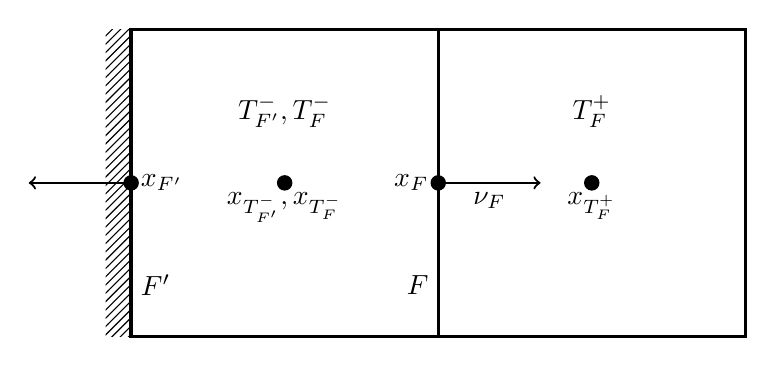
\begin{tikzpicture}[scale=1.3]
\draw[draw=none,pattern=north east lines] (-0.25,0)  rectangle (0,3);
\draw[very thick] (0,0)  rectangle (6,3);
\draw[very thick] (3,0) -- (3,3);
\node at (1.5,2.2) {$T_{F'}^-, T_F^-$};
\node at (4.5,2.2) {$T_F^+$};
\draw[fill=black] (1.5,1.5)  circle (0.07);
\node[below] at (1.5,1.5) {$x_{T_{F'}^-}, x_{T_F^-}$};
\draw[fill=black] (4.5,1.5)  circle (0.07);
\node[below] at (4.5,1.5) {$x_{T_F^+}$};
\draw[thick,->] (3,1.5) -- (4,1.5);
\draw[fill=black] (3,1.5)  circle (0.07);
\node[left] at (3,1.5) {$x_{F}$};
\node[below] at (3.5,1.5) {$\nu_F$};
\node[left] at (3,0.5) {$F$};
\draw[fill=black] (0,1.5)  circle (0.07);
\draw[thick,->] (0,1.5) -- (-1,1.5);
\node[right] at (0,1.5) {$x_{F'}$};
\node[right] at (0,0.5) {$F'$};
\end{tikzpicture}\hspace{0.1\textwidth}
\end{center}
$\mathcal{F}_h^i=\{F_1,\ldots,F_N\}$ is the set of {\em interior intersections}\\
\medskip
$\mathcal{F}_h^{\partial\Omega}=\{F_1,\ldots,F_L\}$ is the set of {\em boundary intersections}\\
\medskip
$\mathcal{F}_h^{\partial\Omega} = \mathcal{F}_h^{\Gamma_D}  \cup \mathcal{F}_h^{\Gamma_N}$
\end{frame}

\begin{frame}
\frametitle{Discrete Weak Formulation}
Finite volume methods us the space
\begin{equation*}
W_h = \{w\in L^2(\Omega) \,:\,  \text{$w|_T=$ const for all $T\in\mathcal{T}_h$}\} .
\end{equation*}
then
{\small\begin{align*}
\int_{\Omega} f v \,dx &= \int_{\Omega} [-\Delta u + q(u)] v\,dx
= \sum_{T\in\mathcal{T}_h} v \int_T -\Delta u + q(u) \,dx &&\text{($v$ const on $T$)}\\
&= \sum_{T\in\mathcal{T}_h} \left[\int_T q(u) v \,dx - \int_{\partial T} \nabla u \cdot \nu v \,ds
\right] &&\text{(Gauss' thm.)} \\
&= \sum_{T\in\mathcal{T}_h} \int_T q(u) v \,dx \\
& \hspace{10mm} -\sum_{F\in\mathcal{F}_h^i} \int_F \nabla u \cdot \nu_F \bigl[v(x_{T_F^-}) - v(x_{T_F^+})\bigr] \,ds \\
& \hspace{10mm}-\sum_{F\in\mathcal{F}_h^{\partial\Omega}} \int_F \nabla u \cdot \nu_F \,ds .
&&\text{(rearrange)}
\end{align*}}
\end{frame}

\begin{frame}
\frametitle{Finite Volume Scheme}
Now approximate the directional derivative
$$\nabla u\cdot \nu_F \approx \frac{u_h(x_{T_F^+})-u_h(x_{T_F^-})}{\|x_{T_F^+} - x_{T_F^-}\|}$$
and the integrals
$$\int_T f \,dx \approx f(x_T)|T| $$
to get the abstract problem
\begin{equation*}
\boxed{ \text{Find $u_h\in W_h$ s.t.:} \quad r_h^{\text{CCFV}}(u_h,v) = 0 \quad \forall v \in W_h }
\end{equation*}
where the residual form \ldots
\end{frame}

\begin{frame}
\frametitle{Residual Form}
\ldots is
\begin{equation*}
\begin{split}
r_h^{\text{CCFV}}(u_h,v)
& = \sum_{T\in\mathcal{T}_h} q(u_h(x_T)) v(x_T) |T|
- \sum_{T\in\mathcal{T}_h} f(x_T) v(x_T) |T|\\
&\ - \sum_{F\in\mathcal{F}_h^i}
\frac{u_h(x_{T_F^+})-u_h(x_{T_F^-})}{\|x_{T_F^+} - x_{T_F^-}\|}
\bigl[v(x_{T_F^-}) - v(x_{T_F^+})\bigr] |F|\\
&\ + \sum_{F\in\mathcal{F}_h^{\partial\Omega}\cap\Gamma_D}
\frac{u_h(x_{T_F^-})}{\|x_{F} - x_{T_F^-}\|} v(x_{T_F^-}) |F| \\
&\ - \sum_{F\in\mathcal{F}_h^{\partial\Omega}\cap\Gamma_D}
\frac{g(x_{F}))}{\|x_{F} - x_{T_F^-}\|} v(x_{T_F^-}) |F| \\
&+ \sum_{F\in\mathcal{F}_h^{\partial\Omega}\cap\Gamma_N} j(x_{F}) v(x_{T_F^-}) |F| .
\end{split}
\end{equation*}
\end{frame}

\begin{frame}
\frametitle{Remarks on the Residual Form}
\textit{Five} different types of integrals are involved in the
residual form:
\begin{enumerate}
\item Volume integral depending on trial and test function.
\item Volume integral depending on test function only.
\item Interior intersection integral depending on trial and test function.
\item Boundary intersection integral depending on trial and test function.
\item Boundary intersection integral depending on test function only.
\end{enumerate}
Dirichlet as well as Neumann boundary conditions are built weakly into the
residual form!\\
\medskip
No constraints on the function space are necessary in this case\\
\medskip
Can be extended to discontinuous Galerkin methods
\end{frame}

\begin{frame}
\frametitle{General Residual Form}
A residual form in PDELab has the following structure:
\begin{equation*}
\begin{split}
r(u,v) &=
\sum_{T\in\mathcal{T}_h} \alpha_T^V(R_T u, R_T v)
+ \sum_{T\in\mathcal{T}_h} \lambda_T^V(R_T v) \\
&\qquad+ \sum_{F\in\mathcal{F}_h^i} \alpha_F^S(R_{T_F^-} u,R_{T_F^+} u, R_{T_F^-} v, R_{T_F^+} v)\\
&\qquad+ \sum_{F\in\mathcal{F}_h^{\partial\Omega}} \alpha_F^B(R_{T_F^-} u, R_{T_F^-} v)
+ \sum_{F\in\mathcal{F}_h^{\partial\Omega}} \lambda_F^B(R_{T_F^-} v) .
\end{split}\label{eq:GeneralResidualForm}
\end{equation*}
which results in the following methods on the local operator
\begin{center}
\tiny
\begin{tabular}{l|l|l|l}
    & volume & skeleton & boundary \\
\hline
residual    & \lstinline!alpha_volume! & \lstinline!alpha_skeleton! & \lstinline!alpha_boundary! \\
                & \lstinline!lambda_volume! & & \lstinline!lambda_boundary! \\
\hline
Jacobian  & \lstinline!jacobian_volume! & \lstinline!jacobian_skeleton! & \lstinline!jacobian_boundary! \\
\hline
Jac.  app.  & \lstinline!jacobian_apply_volume! & \lstinline!jacobian_apply_skeleton! &
\lstinline!jacobian_apply_boundary!
\end{tabular}
\end{center}
$\Rightarrow$ There are up to 11 methods on the local operator. The CCFV scheme implements them all!
\end{frame}

\begin{frame}
\frametitle{Implementation Overview}
The tutorial consist of the following files:
\begin{enumerate}[1)]
\item The ini-file
\lstinline{tutorial02.ini} holds parameters
which control the execution.
\item The main file \lstinline{tutorial02.cc} includes the necessary C++,
DUNE and PDELab header files;
contains the \lstinline{main} function;
instantiates DUNE grid objects and calls the \lstinline{driver} function.
\item File \lstinline{driver.hh} instantiates the PDELab classes
for solving a nonlinear stationary problem with the cell-centered finite
volume method and solves the problem.
\item File \lstinline{nonlinearpoissonfv.hh} contains the class
\lstinline{NonlinearPoissonFV} realizing a PDELab local operator
\item File \lstinline{problem.hh} contains a parameter class which
encapsulates the user-definable part of the PDE problem
\end{enumerate}
\end{frame}

\end{document}

